\documentclass[12pt, a4paper]{article}
\usepackage{graphicx}
\usepackage{amsmath}


\begin{document}
\title{Sea-ice Flow Simplified}
\author{Kecheng Zhang}
\maketitle


\section{Introduction}
Se-ice flow is the study of the movement of sea ice. It is an important topic in the study of climate change. The movement of sea ice is affected by many factors, such as wind, ocean currents, and temperature.
This project aims to model the movement of sea ice using a feed forward neural network. The model is trained using the data of the speed of the piece of sea ice at different positions. The model is then used to predict the movement of the sea ice over a period of time.
This paper will first introduce the mathematics behind the model, then the neural network structure, and finally the performance of the model.
\section{Method}

\subsection{Mathematics}
The speed of the piece can be modeled as
$$ U = 0.5 + 0.3sin(2 \pi x) $$
where x is the position of the piece, and we have data
$x_1(0) = 0.3$, $x_2(0) = 0.7$, and $v_1(0) = v_2(0) = 0$.
We want to calculate
$x_k(t_j)$ and $v_k(t_j)$ for $k = 1, 2$ and $j = 1\dots10000$, where
$\delta t = 10^{-3}$ and $t_j = \delta t j$, such that
$$\begin{cases}
    \frac{\partial x_k}{\partial t} = v_k\\
    \frac{\partial v_k}{\partial t} = (u - v_k) |u - v_k|\\
    \end{cases}$$
and $$ \frac{x_k(t_{j+1}) - x_k(t_j)}{dt} = v_k(t_j)$$

\subsection{Neural Network}
The neural network is a feed-forward network with 2 hidden layers shown in Figure 1. The loss funciton used to train the model is $$\Sigma^2_{k=1}(x_k - x_{k,in} - v_k\delta t)^2$$

\begin{figure}
    \centering
    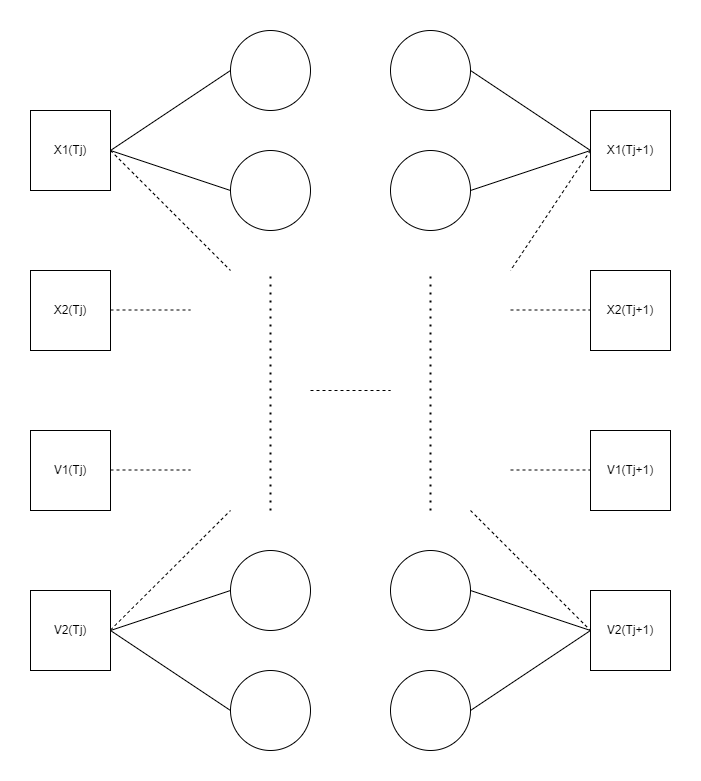
\includegraphics[scale=0.5]{../NN_graph.png}
    \caption[]{Neural Network structure}
    \label{fig:neural_network}
\end{figure}

\section{Discussion}
\subsection{Performance}
The performance of the feed forward neural network was evaluated based on its ability to replicate the physical behavior of sea-ice flow over a specified time frame, which has shown both significance and challenges. 

The model requires little computational resources, and is capable to model the sea-ice flow with good accuracy in short amount of time. However, the error accumulates which leads to a reduction in accuracy as time increases.

Figure 2 and 3 shows the training loss and tesing loss respectivly. Both of the two graphs has shown a increasing trend due to the accumulation of the error in each time step. The training loss increases slower as time increases, which suggests the model converges. While the testing loss suggests the model might be over-fitting. Figure 4 shows the mean square error in training (0.008) and testing (0.531).

\begin{figure}
    \centering
    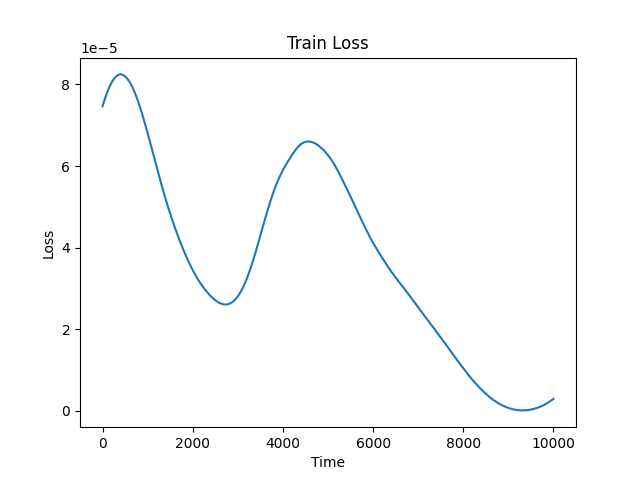
\includegraphics[scale=0.6]{../Train_loss.png}
    \caption[]{The training loss}
    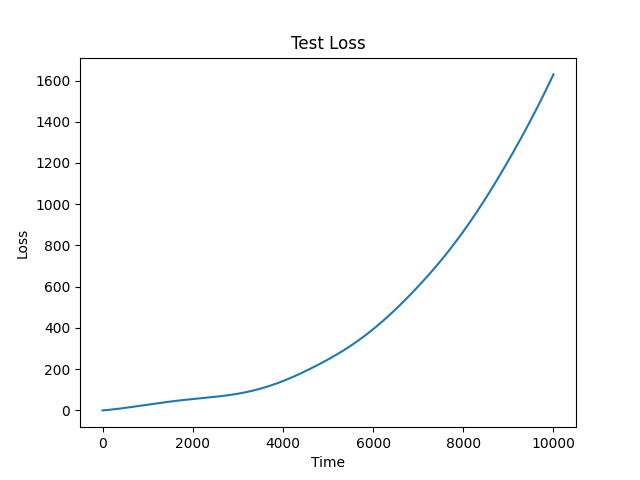
\includegraphics[scale=0.6]{../Test_loss.png}
    \caption[]{The testing loss}
    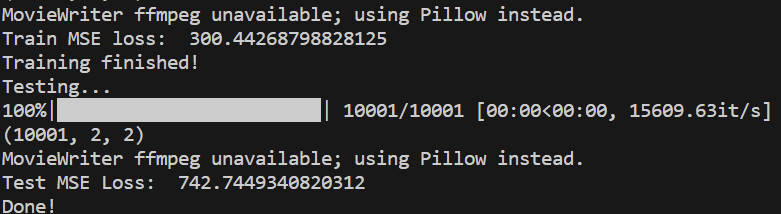
\includegraphics[scale=0.8]{../mse.png}
    \caption[]{MSE}
    \label{fig:loss}
\end{figure}

\subsection{Challenges}
It can be observed that the model suffers heavily from the error accumulation since the calculation of each state relies on the previous state. To solve the issue, there are several possible solutions. Such as enriching the data, performing cross validation, using smaller time setps, and penatize cumulative error. In addition, periodically resetting and retrainig the model is also expected to reduce the error since the model will predict the states in a short future. 

There are also alternative aspects worth investigating to improve the performace of the model. Further reseach include investigating a mroe complex architecture, incoorporating more numerical methods and physical laws.

\section{Conclusion}
In conclusion, the feed forward neural network is capable to model the sea-ice flow with good accuracy in short amount of time. However, the error accumulates which leads to a reduction in accuracy as time increases. Further research is required to improve the performance of the model.

\end{document}